\chapter{Data exploration}
Here I describe the various data exploration techniques I have used. Lots of nice graphs. PCA. Boxplots. Feature plots. Scatter Plots. Unique Values. Is it discrete, binary, continuous.

\section{A note about Test data, training data}

\section{Calculating common statistics}
To start the data exploration, four common statistics, namely the mean, min, max and standard deviation, of every feature across the whole dataset was calculated. The standard deviation was calculated as (with $n$ equal the total number of rows in the dataset, and $x_i$ equal to the $i$'th value of any of the features)
\[
    s = \sqrt{\frac{\sum_{i=1}^n (x_i-\bar{x})^2}{n}}
\]
The source code for the calculations can be found in \appref{source-common-statistics} and all results in \appref{result-common-statistics}. Most results did not tell that much, but a few results stood out. These are shown in table~\ref{tbl:summary-stats-highlights}.
\begin{table}
    {\small\sffamily
        \begin{python}
            import scripts.commonstats_table as c; c.render('../sessions/9-data-exploration/src/summary_statistics.json', ['V5', 'V7', 'V9', 'E9', 'P8', 'P6', 'IsAlert'])
        \end{python}
    }
    \caption{Highlights from the results of the summary statistics. See~\appref{result-common-statistics} for all results.}
    \label{tbl:summary-stats-highlights}
\end{table}
The table shows that the features \fn{P8}, \fn{V7} and \fn{V9}, are zero throughout the whole dataset, and can be ignored. The features \fn{E9} and \fn {V5}, could be binary, but that is only speculation at the moment. Finally the feature \fn{P6} has a mean of 843.73 and a standard deviation of 2795.32, but its maximum is 228812.00, which is many, many standard deviations away from the mean. This could be a sign of some serious outliers, but it could as well be a single trial with a mean far from the other trials. Further investigation are needed to conclude anything here. Finally it is seen that the mean of the \fn{IsAlert} feature is only a little above 0.5, and therefore only a little over 50\% of the time are the drivers alert. This may be a bit surprising. \par
The results of this first step have been to exclude a few features, and get some rough ideas about the shape of some other features. It is now time to resally get to know the different features.

\section{Determining the datatype of features}
Since Ford would not disclose any information about the different features, it is important to get a good picture of which features are discrete/categorical and which features are continous. A natural first step to learn the datatype of the features, is to calculate the number of unique values each feature takes.
\subsection{Unique values}\label{sec:unique-values}
It requires a little thought to pinpoint exactly what needs to be calculated. On one hand it is natural to calculate the number of unique values a feature takes across the whole dataset. On the other hand it could happen, that a discrete feature might have only (eg.) 3 unique value within any trial, but the values differ between various trials. This way we would have a feature with 1500 unique values across the whole dataset, but with max 3 unique values within any given trial. Therefore the number of unique values within a trial are calculated for every feature and every trial. Based on this result, the minimum and maximum number of unique values within a single trial, is calculated for every feature. The source code can be found in \appref{source-unique-values} and results are shown in table~\ref{tbl:result-unique-values}.\mytodo{The result table in appendix or in report?} \par
\begin{table}
    {\small\sffamily
        \begin{python}
            import scripts.uniquevalues_table as c; c.render(['V7','V9','P8'])
        \end{python}
    }
    \caption{The minimum and maximum number of unique values within the trials, for every feature in the dataset. Also the total number of unique values for each feature, across the whole dataset, are shown.}
    \label{tbl:result-unique-values}
\end{table}
A couple of things should be noticed about the results. Almost all features have som trials where they only take on one unique value. For categorical features, this could be perfectly normal, but for a continous feature it seems to be pretty unlikely to have only one value in a trial spanning two minutes. Is a feature, that in some trials seems continous, but then only have one value in other trials, just turned off in the latter trials? And how should the feature be handled in trials where it is ``off"?. This discussion is continued in section~\ref{sec:outlier-detection} about outlier detection. \par

From table~\ref{tbl:result-unique-values} it is also seen, that only features \fn{P1}, \fn{P2} and \fn{V11} is consistently having lots of unique value, across all trials. It seems fair to call these features continous. Feature \fn{V1} have some trials where it takes on 969 different values, but it also have trials with only one unique value. Across the whole dataset it takes on 12374 unique values. This could be explained by feature \fn{V1} being continous in a small number of trials (about 15-30), and turned ``off" in all other trials. Further exploration will show whether it is true or not. \par

Another interesting detail is that there are two pairs of features ((\fn{P3},\fn{P4}), (\fn{P6},\fn{P7})) in the results, that share exactly the same number of unique features. Both min and max and total. This indicates a possible relationship between the features, and later (section~\ref{sec:scatterplots}) it is shown that this is in fact true. \par

A final remark about the number of unique values, is that feature \fn{E9} and \fn{V5} indeed are binary. Also if a limit of max 40 unique values within a single trial is set, as an indicator for categorical features, \fn{E3}, \fn{E7}, \fn{E8}, \fn{V3} and \fn{V10} are seen to be categorical. \par

\subsection{Plotting some features}
To get a more nuanced picture of the various features, it is now time to visualize the data. The first thing of interest is to plot every feature for a couple of trials, to see the structure of the features, and how much they vary between different trials. For a start some random plotting was done in the interactive ipython-shell\footnote{For details about the software setup used, see chapter~\ref{chp:tools}}. \par
\begin{figure}[!hbtp]
    \centering
        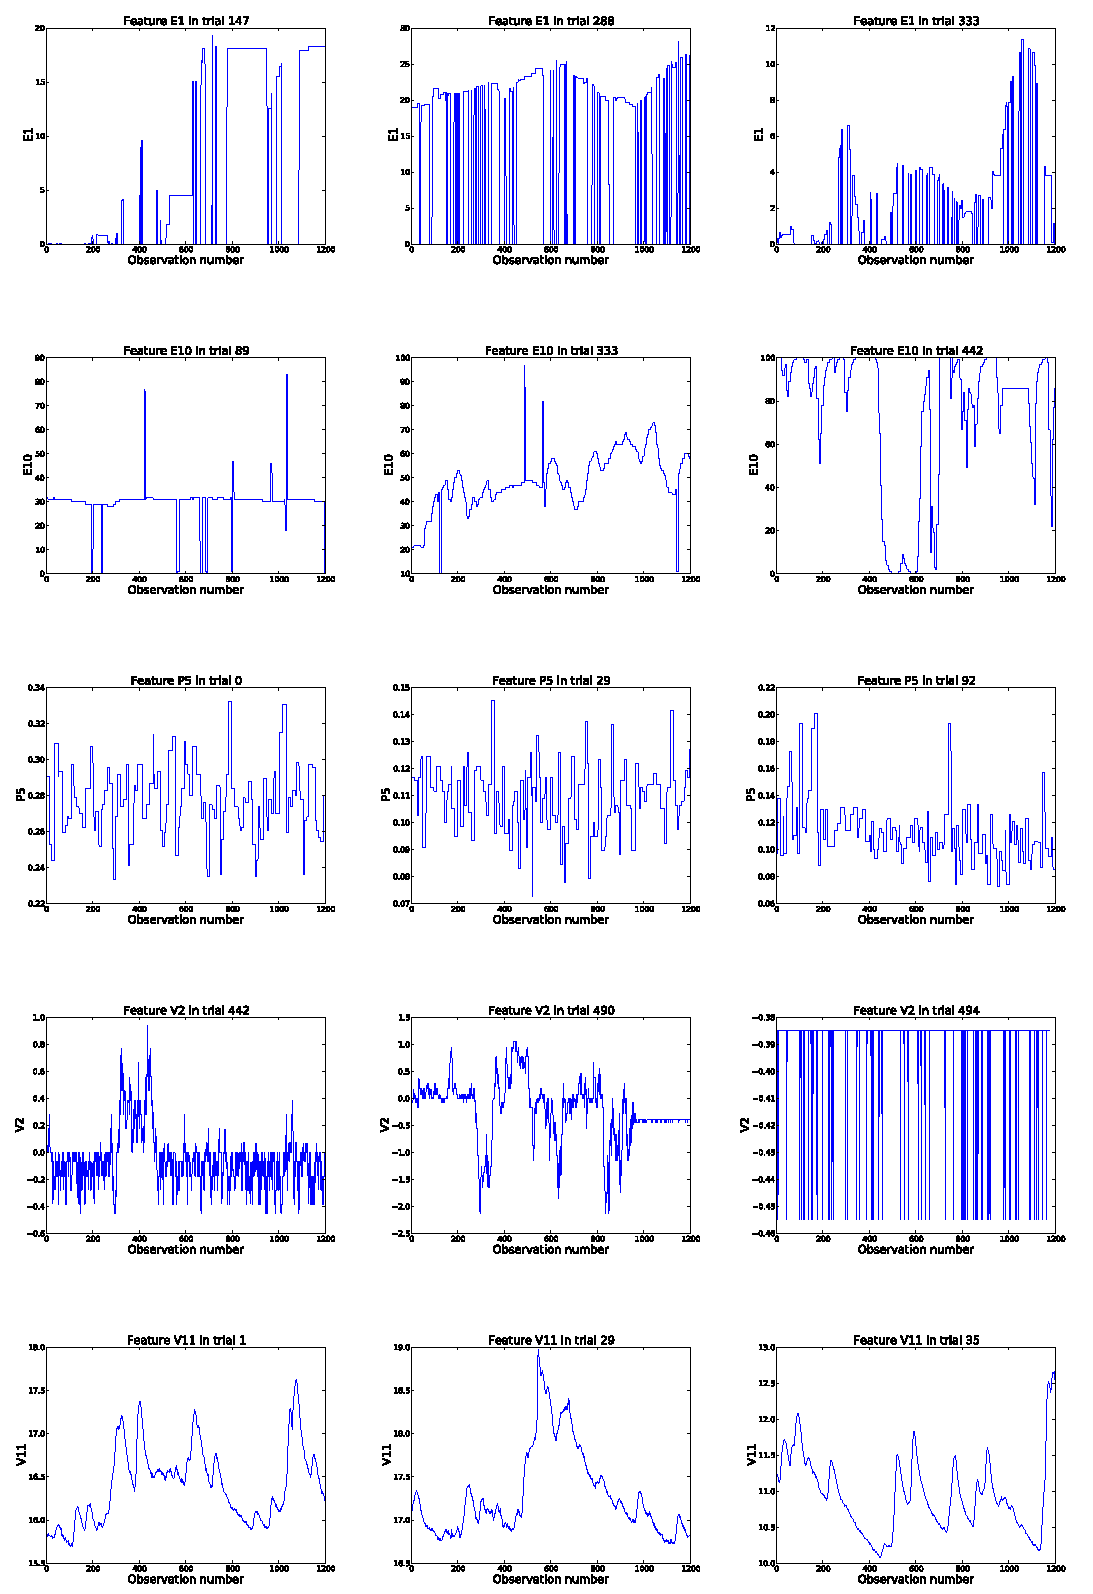
\includegraphics[width=\textwidth]{media/feature-plots-sheet.pdf}
    \caption{A caption}
    \label{fig:exploratory-feature-plots}
\end{figure}
The main result from the introductory plotting of features is that: a feature varies alot in structure between different trials, many features are just one value in some trials (was already shown in section~\ref{sec:unique-values}), some features deviates a lot from their ``normal" structure, in a few trials (more about that in section~\ref{sec:outlier-detection} about outliers). Above all, the main conclusion from the plots is that the data quality could be better.


\section{Outlier detection}\label{sec:outlier-detection}
Broader view than 95\% percentile. Trial with only IsAlert=0 outlier? Maybe mention troubles with defining outlier? Theorem in book Duda.
\subsection{Making boxplots of features}

\section{Finding possible discriminating features}
\subsection{Testing binary features}
\subsection{Scatterplots}\label{sec:scatterplots}
\subsection{Making a Principal Component Analysis}
Giver det mening på binære variable?

\section{Conclusions}
